\documentclass{article}
\usepackage[utf8]{inputenc}
\usepackage{amsmath}
\usepackage{amsfonts}
\usepackage{amssymb}
\usepackage{graphicx}
\graphicspath{ {Images/} }
\usepackage{float}
\usepackage[backend=bibtex,style=verbose-trad2]{biblatex}
%\bibliography{bib}

\begin{document}

\title{Employee Attrition: What makes an employee leave?}
\author{
	Christopher Boomhower$^1$
	\and
	Stacey Fabricant$^2$
	\and
	Alex Frye$^1$
	\and
	David Mumford$^2$
	\and
	Michael Smith$^1$
	\and
	Lindsay Vitovsky$^1,^2$
}
\date{}
\maketitle{}

\begin{center}
{$^1$ Southern Methodist University, Dallas, TX, US\\$^2$ Penn Mutual Life Insurance Co, Horsham PA}
\end{center}

%definition of quote with addition of [\textbf{Abstract --- ]
\renewenvironment{abstract}
               {\list{}{\rightmargin\leftmargin}%
                \item[\textbf{\hspace{10mm}Abstract ---}]\relax}
               {\endlist}



\begin{abstract}\noindent In this paper, we present a model for employee attrition prediction and discuss the ethical impacts of using such a model within private and public sector organizations. As it is in Human Resource personnel’s best interest to improve retention, implementing statistical and machine learning techniques is the most viable means to attrition abatement. To this end, we examine Office of Personnel Management public sector, Bureau of Labor Statistics public sector, and IBM anonymized private sector employee separation data. Three classification models (Methodologies include Logistic Regression, Random Forest, and K Nearest Neighbor) are trained and tested on these data before selecting our best fit model for attrition prediction. We finally use metrics such as Gini and Permutation Importance to identify the most impactful variables in determining prediction outcome before presenting the ethical ramifications of using such outputs in HR planning. [WILL ADD SENTENCE FOR MAIN RESULT AND SENTENCE FOR MAIN CONCLUSION ONCE THESE DEVELOPMENTS ARE COMPLETE].\end{abstract}

 
\section{Introduction}

\paragraph{How much does it really cost to lose an employee? Studies such as the Center’s for American Progress analysis (November, 2012) indicate a separated employee may cost anywhere between 16 percent to 213 percent depending on the position [1]. Precisely quantifying this may seem out of reach depending on the complexity of a particular role, but areas of impact that one may foresee at many organizations are: 1) determining if the employee’s vacancy should be replaced or duties handed off to others; 2) posting the job opportunity to various outlets; 3) interviewing, hiring, and training a replacement; 4) enduring lowered employee morale / possible lower productivity from remaining employees; and 5) tolerating a lower skill set from an underdeveloped replacement [2].}

\subparagraph{Corporations are keenly aware of the downsides to losing employees and exert great effort to maintain retention levels. In their efforts to not only attract talented workers but retain them as well, businesses provide substantial benefits [3]. With industry competitiveness the norm, many employers may still face retention challenges as their employees have alternate employment options. To become even more proactive in attrition prevention, companies must gain a solid understanding for the reasons their employees separate. Foresight into attrition development and contributing factors empowers Human Resource departments to improve retention efforts through improved planning and intervention. While such insights are available to organizations that store employee data, these understandings are not within reach without sufficient analysis.}

\subparagraph{The first step in gaining foresight into employee attrition is obtaining pertinent data. Companies are understandably reluctant to release the methods, proprietary or purchased, that use even anonymous data to help them in their management of human resources. Various articles allude to this challenge [4, 5, 6]. However, we identified three valid sources of Human Resources data in the forms of Office of Personnel Management data, Bureau of Labor Statistics data, and the “IBM HR Analytics Employee Attrition” dataset. All three forms were analyzed in unison to complement one another in insight and model validity.}

\subparagraph{During analysis, dimensionality reduction was performed on the datasets. This was essential to reduce numerous correlating and covariant relationships present between dataset variables. Only after these relationships were addressed and the datasets simplified were the data prepared for modelling.}

\subparagraph{[ADD PARAGRAPH ABOUT MODELLING PHASE AS PROJECT DEVELOPMENT PROGRESSES][ADD PARAGRAPH SUMMARIZING MAIN RESULTS AS PROJECT DEVELOPMENT PROGRESSES][ADD PARAGRAPH SUMMARIZING MAIN CONCLUSIONS AS PROJECT DEVELOPMENT PROGRESSES][ADD PAPER OVERVIEW PARAGRAPH ONCE REMAINING PAPER CONTENT FILLS IN]}
  
\section{Attrition as Seen in Civil Service Workers}

\paragraph{The U.S. Office of Personnel Management (OPM) serves as the central Human Resources department for all Federal agencies, including the management of federal agency health insurance and retirement benefits. Their oversight of policy implementation as well as being a general resource for all agency Human Resource departments makes their employment data of particular interest for this paper. OPM releases on a quarterly basis updated separation data on its over two million federal civil service workers.  We used these anonymized data sets to create a full year of separation data, spanning October 2014 - September 2015.   These data [7], include the following variables: 1) age group, captured categorically in 5 year increments (AGELVL and AGELVLT), 2) agency type and subtype information (AGYTYP, AGYTYPT, AGY, AGYT, AGYSUB, and AGYSUBT), 3) gender (GENDER and GENDERT), 4) General Schedule Grade, or equivalent, dictating salary level (GSEGRD, 5) geographical location of the employee down to the state level (LOCTYP, LOCTYPT, LOC, LOCT), 5)length of service as a government employee captured in one year increments until five years was achieved, then every five after that (LOSLVL and LOSLVLT), 6)occupation type  in regards to white or blue collar, occupation family, and in some cases, down to the particular occupation itself (i.e. "chaplain") (OCCTYP, OCCTYPT, OCCFAM, OCCFAMT, OCC, OCCT), 7) occupation category among seven main categories (i.e. "Technical" and "Clerical")(PATCO and PATCOT), 8) pay plan and grade for both GSE and non-GSE occupations (PPTYP, PPTYPT, PPGROUP, PPGROUPT, PAYPLAN, PAYPLANT, and PPGRD), 9) salary range, captured categorically starting with $<$ \$20,000 and followed in \$10,000 increments (SALLVL and SALLVLT), 10) reason for separation (SEP and SEPT), and 11) type of appointment and worschedules, denoting factors such as permanence, seasonality, and executive status (TOATYP, TOATYPT, TOA, TOAT, WSTYP, WSTYPT, WORKSCH, and WORKSCT).   }


\subparagraph{There are certain points worth noting to understand our findings in the correct context.  The General Schedule Pay Scale is the centralized pay scale used by many civil service agencies. Whether or not a person is paid under the GS, the OPM converts the level he or she is paid under to the GS for data collection purposes. The scale numbers 1-15 and there are ten “steps” within each of those levels.  Also, to remain competitive with industry salaries, the GS operates a locality adjustment scale that adds a particular percentage to a person’s salary, based on city of occupation alone.}

\subparagraph{ Also, beginning on January 1, 1987,  new civil service employees were paid under the Federal Employees Retirement System (FERS). This mix of Social Security, a Basic Benefit Plan, and a Thrift Savings Plan helps make civil service positions stand out from many current private sector jobs in terms of retention. We account for this factor in our research, taking into consideration the confounding effect this has on length of service (LOS). At the time of this paper, the pension is based on salary and length of service.}


\section{OPM Data Consolidation, Sampling, \& New Attributes}

\paragraph{Our research focuses on the following employee types, only using observations that fit the following rubric: 1) domestic workers (no international positions), 2) employees aged 20 and greater, 3)employees with a job grade level greater than 7 (i.e. white collar only), and only those who are considered full-time employees (i.e. no contracted, temporary, or part-time employees).}  
  
 
\subsection{Data Removal}

\subparagraph{After reviewing the percentage representation of the various occupation types, as well as investigating the types of jobs that comprise each grouping, we kept only Professional and Administrative positions. Fig. 1 depicts the overall record counts present within our dataset by occupation category type. As observed, there are more employees of Administrative and Professional occupation types than any other category. Reviewing separation type ratios which comprise these total counts provides further insight and justification into why Professional and Administrative jobs are targeted within this paper.}
 
 
\begin{figure}
\caption{Fig. 1. Occupation Category Type – Observation Counts}
\end{figure}
 
\subparagraph{The percentage plot of Fig. 2[Field] indicates the distribution of separation types within each occupation category. Note for improved granularity, non-separated employee data has been removed from the visualization as there are far more employees remaining at work than there are leaving, which therefore skews plotted results. So, only true separations are represented visually.}

\begin{figure}
\caption{Fig. 2. Occupation Category Type – Separation Percentages with NS Removed}
\end{figure}
 
\subparagraph{As Fig. 2[Field] illustrates, approximately the same number of Professional employees who retired (SD) in this timeframe quit (SC) as well. Treating retirement as a proxy indicator for retention, this even distribution of quits vs. retirements suggests great retention rates among Professional employees and aligns with non-separation counts as well. Similar argument is to be made of Blue Collar jobs also, and the combination of individual transfers out (SA) and quits is approximately the same in size as retirements for Administrative types. However, the Professional category type was identified as a better candidate for primary model application due to its large total count, as discussed previously, in combination with its more widely diverse professional job types that more closely resemble private sector occupations. Nonetheless, due to its high employee count, strong retention numbers, and similar transfer and quit counts compared to retirements, the Administrative occupation category was selected as secondary target for modeling purposes as will be discussed further in section 5. Therefore, data for all occupation category types, except Professional and Administrative, were removed from our dataset.} 
 
 
\subsection{OPM Computed Attributes}

\paragraph{Six new attributes were created through aggregation or calculation: 1) SEP Count by Date \& Occupation – Total number of separations (of any type) for a given Date and Occupation; 2) SEP Count by Date \& Location – Total number of separations (of any type) for a given Date and Location; 3) Industry Average Salary – Average salary amongst non-separated employees, grouped by quarter, occupation, pay grade, and work schedule; 4) Lower Limit Age – Youngest age within each age level category; 5) Years to Retirement – Based on FERS retirement eligibility baseline of 57 years of age [8]; and 6) Salary Over/Under Industry Average – Difference between computed average salary of non-separated employees and actual salary for each observation. Note also another 1,293 observations were removed after calculating industry average salary as they had no matching non-separation observations (matched on quarter, occupation type, pay plan /grade, and work schedule), which were utilized to ensure realistic salary averages.}
 
\subsection{Bureau of Labor Statistics Derived Attributes}

\paragraph{In addition to the OPM data, we merged 10 attributes from the Bureau of Labor Statistics (BLS). Data were sourced from Federal Government industry codes across all regions. Although assumed to be highly correlated, we sourced both Level (Total number) and Rate (Percentage of Level to total employment and / or job openings) for the following statistics: 1) Job Openings, 2) Layoffs, 3) Quits, 4) Total Separations, and 5) Other Separations. While Rate paints an aggregated, holistic picture for job market trends, Level provides a raw count for total separations alone. Both these statistics were captured by a monthly aggregate and merged to the OPM data by their respective months.}
 
\subsection{Sample Design}

\paragraph{From an original 8,423,336 observations, we ultimately result in two datasets for Professional and Administrative occupations, reduced to 1,282,291 and 2,128,093 observations respectively. Of the 1,282,291 observations present in the reduced OPM dataset of professional occupations, only 23,008 contained actual separation data and all other observations were considered non-separation. This state of data was inoperable for analysis; therefore, a sample design was determined to mitigate sample size constraints and high variance amongst frequencies of separation types.}
 
\subparagraph{Data were divided into groups based on separation type, allowing a maximum of 4,000 observations per type to persist forward during analysis. In so doing, the following retirement separation types were combined: 1) SD Retirement – Voluntary, 2) SE Retirement – Early Out, 3) SF Retirement – Disability, and 4) SG Retirement – Other. Next, the following separation types were dropped completely: 1) SB Transfer Out – Mass Transfer, 2) SK Death, 3) SL Other Separation, and 4) SJ Termination (Expired Appt/Other).}
 
\subparagraph{Within each separation group (including non-separation), proportional allocation was performed on a combination of date and age level strata to ensure a sample demographic which, as closely as possible, represents that of the original strata-level populations. After sampling, we were left with 16,638 observations in our primary dataset for model generation. The secondary dataset of Administrative occupations also contained these unbalanced strata, and thus the same sample design was implemented to reduce the dataset further to 17,238 observations.}
 
\section{Preliminary Analysis}

\paragraph{Reviewing the final Professional occupation category data provided lead indicators that assisted us in creating our primary attrition model. The findings described below guided our approach to model generation as they suggest some attributes do truly correlate more strongly with attrition than others. These findings also serve as primer to our feature importance analysis as will be described in Section 5.}
 
\begin{figure}
\caption{Fig. 3. Numeric Attribute and Separation Type Correlation Matrix}
\end{figure}
 
\subparagraph{As indicated in Fig. 3, there are several intuitive observations to be made of the correlation values shared by separation type and the remaining quantitative attributes present in the dataset. Note numerical values shown are Pearson’s correlation coefficient values. Separation due to voluntary retirement (SEP\_SD) is positively correlated with paygrade (r = 0.2), salary differential from the industry (r = 0.3), and length of service (r = 0.6). Even though these are to be expected, this is still worth noting as it supports the idea that the prospect of retiring with benefits, as opposed to quitting, can help entice an employee to stay. Of course, the pension calculation is heavily based on number of years of service, so it is unsurprising that length of service is the highest positively correlated factor for separation by voluntary retirement.}
 
\subparagraph{The correlation values for separation from quitting (SEP\_SC) in Fig. 3 is what interests us most.  As paygrade decreases, the likelihood of separation by quitting increases (r = 0.2). This make logical sense, as paygrade is directly tied to income.  However, this correlation also exactly matches the correlation for the salary differential from the industry, so there is not enough direction to say that the status of the paygrade is what matters more so than the actual salary. Though not indicated in Fig. 3, salary and paygrade level do in fact strongly correlate with one another (r = 0.9). As such, the two are most likely one and the same in an employee's mind, and only one of the two will be used for modeling purposes.}
 
\subparagraph{Finally, the correlation of quits to years until retirement eligibility is positively correlated (r = 0.3), whereas it is negatively correlated with length of service (r = -0.4); the further someone is from being able to retire, the more likely they are to quit. But when considering the correlations observed for paygrade and salary differential, a key takeaway is that the job positions for which it is more difficult to replace and train should be assigned higher paygrades and lower income differentials from industry. This conclusion aside, these insights solidified our data as being predictive of attrition.}

\subparagraph{[WILL DESCRIBE CATEGORICAL DATA RELATIONSHIPS WITH SEPARATION]}

\section{Modeling and Evaluation}

\paragraph{Methodologies Logistic Regression, Random Forest, and K Nearest Neighbor(KNN) were implemented to predict separation types amongst our sampled professional occupations. Four disparate feature input selections were utilized in attempts to reduce dimensionality in our initial input of 99 attributes. Ultimately, Logistic Regression produced most effective trained results and the generated models were applied to a different demographic of Administrative occupations.}
 
\subsection{Feature Input Selections}

\paragraph{Four feature input selections were made during the modeling process in search of the best features for each model type individually. Selections made were: 1) Full 99 Raw Scaled Value Features; 2) Principal Component Analysis(PCA) Eigenvector Matrix; 3) Top 15 Raw Scaled Features within Each PCA Loading; 4) Manual Logistic Regression Feature Selection.}

\subparagraph{Full 99 Raw Scaled Value Features: All 99 values after Min Max Scaling was performed.}

\subparagraph{Principal Component Analysis(PCA) Eigenvector Matrix: Principal component analysis was performed on our professional occupation samples in attempts to reduce our 99 input attributes. As can be seen in Figure ~\ref{fig:PCA_Scree_CumVar}, the percentage of explained variance leveled out around 22 components, at which point cumulative explained variance approached 80\%.}

\subparagraph{}
\begin{figure}[H]
\centering
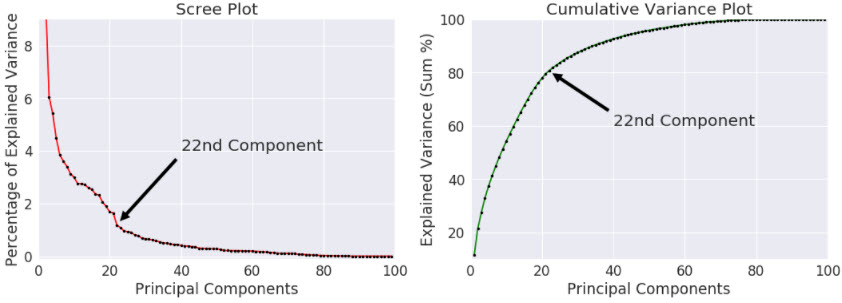
\includegraphics[width=\linewidth]{PCA_Scree_CumVar.jpg}
\caption{Explained and Cumulative Variance Plots}
\label{fig:PCA_Scree_CumVar}
\end{figure}


\subparagraph{These 22 principal components were utilized both as a dataset of component vectors as well as to identify the top 15 features within each of the 22 component loading magnitudes. The latter approach reduced our inputs to 49 features, allowing only the most important features to proceed into our model as raw scaled values, based on PCA component loadings.}

\subparagraph{Manual Logistic Regression Feature Selection:[CHRIS TO WRITE A PARAGRAPH ON THIS PROCESS, WHAT VALUES ARE ANALYZED{P VALUE, VIF, ETC.}, AND THRESHOLDS FOR REMOVAL.]
}
 

\subsection{Classification Model Training and Comparison}

\paragraph{[DISCUSS CV SPLIT FOLDS HERE.....]}

\subparagraph{Among the three model types and four separate input features tested, Logistic Regression with Manual Feature Selection was identified as most effective. As depicted in Table ~\ref{fig:AccTable} the [INTERPRET MODEL MEAN ACCURACY RESULTS HERE]} 

\subparagraph{}
\begin{table}[H]
\centering
\caption{Raw Accuracy Data for Top 4 Model Results}
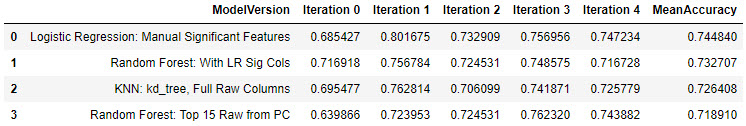
\includegraphics[width=\linewidth]{AccTable.jpg}
\label{fig:AccTable}
\end{table}

\begin{figure}[H]
\centering
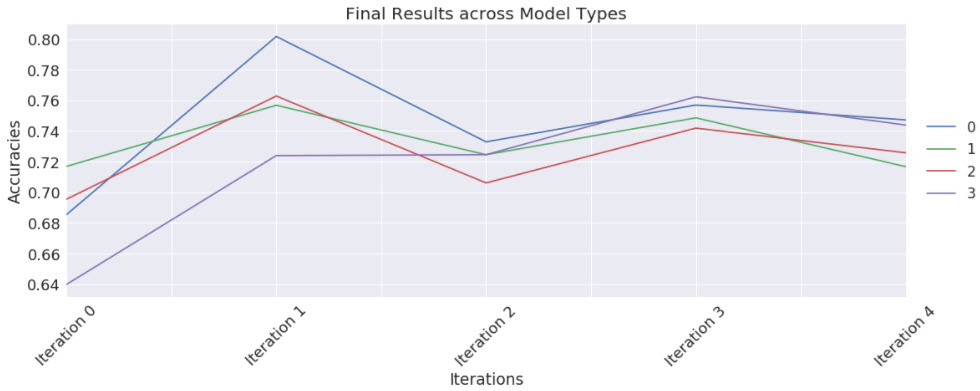
\includegraphics[width=\linewidth]{AccPlot.jpg}
\caption{Accuracies Across Test Folds for Top 4 Model Results}
\label{fig:AccPlot}
\end{figure}

\subparagraph{Furthermore, we may see visually in Figure ~\ref{fig:AccPlot}, the variation in accuracy for each model across the 5 fold tests further supports the Logistic Regression results as a strong selection.[INTERPRET FOLD ACCURACY METRICS HERE, MAKING NOTE THAT LEGEND INDEXES CORRESPOND TO Table ~\ref{fig:AccTable}]}

\subparagraph{[discuss lr roc plot here.....Figure ~\ref{fig:ROCPlot}.]}

\subparagraph{}
\begin{figure}[H]
\centering
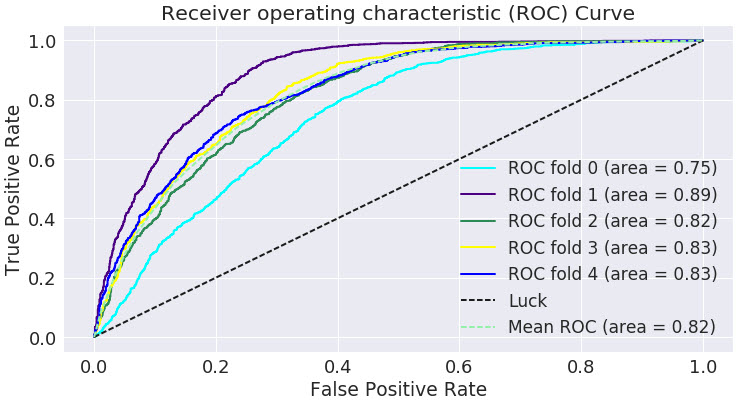
\includegraphics[width=\linewidth]{ROCPlot.jpg}
\caption{Accuracies Across Test Folds for Top 4 Model Results}
\label{fig:ROCPlot}
\end{figure}

\subsection{Feature Importance Analysis}

\paragraph{[CHRIS TO PLACE TEXT HERE.]}


\subsection{Expanding Testing Scope to Administrative Occupations}

\paragraph{[TEXT PLACEHOLDER FOR RESULTS, APPLYING FINAL MODEL ON ADMINISTRATIVE DATA. INCLUDE COMMENTS ON HOW ONE MODEL DOES OR DOES NOT WORK WELL ACROSS INDUSTRIES. ALSO, PROVIDE RESULTS ON EFFECTIVENESS OF THE MODEL, WHEN OCCUPATION FAMILIES ARE INCLUDED AND A SEPARATE MODEL IS GENERATED FOR EACH POPULATION SEGMENT]. Here is a reference to confus matrix... Figure ~\ref{fig:AdminLRConfus}}

\subparagraph{}
\begin{figure}[H]
\centering
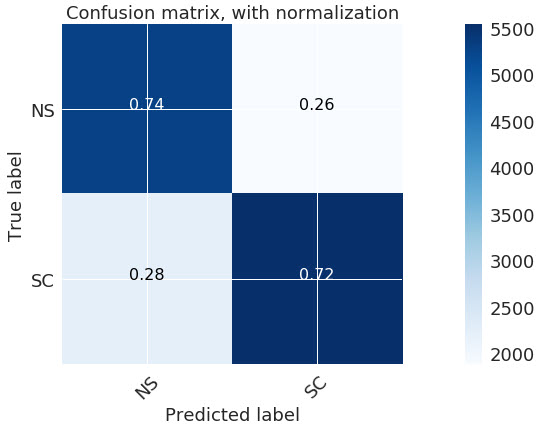
\includegraphics[width=\linewidth]{AdminLRConfus.jpg}
\caption{Confusion Matrix Results for Predicting Administrative Occupations Results}
\label{fig:AdminLRConfus}
\end{figure}

\section{External Validation}

\paragraph{Our model is based on features made public through the Federal Office of Personnel Management and the Bureau of Labor Statistics – as such, we expected to see some limitations in the validity of our model for private sector companies. A part of our concern was in the fact that we would not have additional data that some HR offices might have access to such as self-reporting surveys on job satisfaction, work-life balance, and even performance reviews. In an effort to produce as accurate a model as possible, we sought out other sources that might provide insight into how such variables might impact the attrition rate.}

\subparagraph{IBM released a dataset in 2015 that contains 35 features with a categorical response variable for Attrition as "Yes" or "No" [25]. This dataset is "based [off] real data with all personal identifiers removed," but was "also tweaked so that it performs better in telling a story about attrition” [26]. This data was provided as part of an IBM Watson Analytics promotion to push their new analytics platform. IBM also provided a sample use-case scenario for the dataset wherein they identified the primary features correlated to attrition as well as determined the attrition rate for several demographic categories of employees [27].}

\subparagraph{While it is true this dataset was manipulated in an undescribed fashion, it still provides insight into what data is considered valuable by IBM Watson Analytics in defining and predicting employee attrition. To that end, we performed exploratory data analysis to verify the findings of the IBM Watson Analytics group as well as compare the strongest features of this dataset with the features selected for our model.}

\subparagraph{In Fig. 6 are the results of a simple Pearson's correlation for several features against attrition. The features with the highest correlation are those concerning age, duration of employment, and economic factor such as monthly income and whether the employee participated in overtime. While this wouldn't seem to say that qualitative features such as job satisfaction or work/life balance aren't important in the model, it might lead to economic and duration factors having greater impact – even if individually these features aren't particularly correlated with attrition.}

\begin{figure}
\caption{Fig. 6. IBM Attribute and Separation Correlation Values [PENDING LABEL SIZE AND OVERLAPPING LABEL MODIFICATIONS FOR COMPLETE DRAFT]}
\end{figure}
 
\subparagraph{In comparing these particular features with the data from OPM and BLS, some features show similar correlations to that found in the dataset used for our model. Age having a negative correlation matches up with the trend that younger employees are more likely to separate from the company than their older colleagues. Further, the fewer years spent in the role, the greater the correlation with attrition which is similar, again, to the findings in our analysis of the OPM dataset. Finally, Monthly Income is among the highest correlated features to attrition, once more matching what was observed with the OPM dataset.}
 
\subparagraph{The data provided by IBM may not be definitive in that it's still ultimately a sample dataset that had been "tweaked" despite its origin as anonymized real-world data; however, it may still reflect growing trends in employee retention and attrition. For millennials, 60\% are open to different job opportunities, but 26\% are less likely to leave if they are engaged at their current place of employment [28]. This seems to reflect the fact that, for disengaged employees, 54\% would leave their current position for a pay increase of 20\% or less, whereas only 37\% of engaged employees would do the same [29]. Together with the IBM data, these trends might seem to suggest that while work satisfaction is very important, the decision seems to come down to economic factors – the same factors that we focused on in building our model.}
 
\section{Ethical Considerations}

\paragraph{At the crux of any activity that collects and interprets data on human behavior is the question, “Who is to benefit, the gatherer or the subject?” Would our model prompt a company to strive for increased employee tenure, or would it reduce compensation and other benefits once it is aware of an employee’s “shelf life?” We touch upon several of these ethical dilemmas below.}
 
\subsection{Size of the Interested Party}

\paragraph{One of the benefits of using third party data is that a smaller organization does not risk breaking anonymity. For example, maintaining anonymity in a smaller size company, with only one employee in accounting, would be outside the realm of possibility should the organization gather such data as presented herein on their own employees. However, by using data from such a large entity as the US Government, a Human Resources professional would be able to gain insight about the departments in their company without risking important employee relationships.}
 
\subparagraph{That being said, the data we analyzed is applicable to employee groups as a whole, not individually. There are many factors that could impact an employee choosing to leave, and when big data is applied to small departments or single individuals, an HR professional might incorrectly assume that one of their employees will act similarly to the behaviors of general groups. In reality, an employee’s family life, manager, financial situation, and perception of self-worth may drastically affect the outcome of applying large-scale behavioral models to small populations.}
 
\subsection{Data Collector}

\paragraph{There is no denying that, in the case where employee disclosure is required as part of the data gathering process (i.e. the performance data from the IBM dataset), an employee may not feel comfortable being completely honest about certain attributes. For example, if an employee is to rate their job satisfaction, would said person be concerned that their results would be seen by a manager and used against them? Would the realization that he or she is not satisfied prompt them to then begin a job search?}
 
\subparagraph{We contend that surveying employees (rather than analyzing known facts that are collected by default) are more prone to ethical issues. Certainly, the collection of employee data, such as length of service, years to retirement, etc. are features that are not very attributable to individual respondents. But, data collection that reflects personal feelings (i.e. job satisfaction) or other types of individual metrics (i.e. performance reviews) risk being attributable to specific employees.}
 
\subparagraph{For these reasons, if a company wishes to gain insight into the attrition rate of their own employees, it would be advisable to either 1) form an internal team or committee to monitor and advise on the collection of employee data and 2) perhaps bring in a third-party researcher that will commit to maintaining anonymity and autonomy.}
 
\subsection{Improving the Life of an Employee}

\paragraph{Making inferences of what prompts an employee to leave should be checked against whether the lives of the employees are actually improved. A company that is wanting to simply reduce attrition cost might actually commit unethical acts if they do not take a comprehensive approach to this practice.}

\subparagraph{For example, if gender is collected as part of a survey, perhaps an employee attrition model finds that women have a higher attrition rate than their male peers. If we build our model around that feature, we then are at risk of making the statement that gender is just as important as, say, salary when determining attrition rate. Even though gender may have societal associations that would result in attrition, it would be considered morally reprehensible if those associations were taken into consideration for hiring practices.}
 
\subparagraph{Also, consider the ever elusive “work/home life balance.” If personal events are found to affect employee attrition, then the question becomes, “Is that something that a Human Resources or Management professional should be screening candidates for?” There is a possibility that such data can impact the model, and while there is likely quite a bit of improvement that may come from collecting such data, the risk of bias that could come of it is ever present.}
 
\subsection{Systematic Propagation of Unfair Practices}

\paragraph{A glaring ethical challenge from employing an attrition model is the chance that once trends are seen, a company actually instills processes that create systematic disadvantages for its employees. For example, say a company learns that individuals aged 30-45 years, working in marketing departments, average 3 years at their employer and are often underpaid in relation to their industry when they quit. In response, the company updates its profit sharing plan to only vest for its employees once they have reached 5 years of service. Rather than keep more employees around, the company inadvertently created more discontent, profiting by keeping unvested profit sharing contributions and continuing to pay their workers less than the industry average.}

\section{Conclusion}

\paragraph{[ADD CONCLUSION DETAILS AS PROJECT DEVELOPMENTS COME TO END FOR COMPLETE/FINAL DRAFT]}
 
\section{References}

\printbibliography

\end{document}